\documentclass[11pt,a4paper]{report}
\usepackage[textwidth=37em,vmargin=30mm]{geometry}
\usepackage{calc,xunicode,amsmath,amssymb,paralist,enumitem,tabu,booktabs,datetime2,xeCJK,xeCJKfntef,listings}
\usepackage{tocloft,fancyhdr,tcolorbox,xcolor,graphicx,eso-pic,xltxtra,xelatexemoji}

\newcommand{\envyear}[0]{2025}
\newcommand{\envdatestr}[0]{2025-10-15}
\newcommand{\envfinaldir}[0]{webdb/2025/20251015/final}

\usepackage[hidelinks]{hyperref}
\hypersetup{
    colorlinks=false,
    pdfpagemode=FullScreen,
    pdftitle={Web Digest - \envdatestr}
}

\setlength{\cftbeforechapskip}{10pt}
\renewcommand{\cftchapfont}{\rmfamily\bfseries\large\raggedright}
\setlength{\cftbeforesecskip}{2pt}
\renewcommand{\cftsecfont}{\sffamily\small\raggedright}

\setdefaultleftmargin{2em}{2em}{1em}{1em}{1em}{1em}

\usepackage{xeCJK,xeCJKfntef}
\xeCJKsetup{PunctStyle=plain,RubberPunctSkip=false,CJKglue=\strut\hskip 0pt plus 0.1em minus 0.05em,CJKecglue=\strut\hskip 0.22em plus 0.2em}
\XeTeXlinebreaklocale "zh"
\XeTeXlinebreakskip = 0pt


\setmainfont{Brygada 1918}
\setromanfont{Brygada 1918}
\setsansfont{IBM Plex Sans}
\setmonofont{JetBrains Mono NL}
\setCJKmainfont{Noto Serif CJK SC}
\setCJKromanfont{Noto Serif CJK SC}
\setCJKsansfont{Noto Sans CJK SC}
\setCJKmonofont{Noto Sans CJK SC}

\setlength{\parindent}{0pt}
\setlength{\parskip}{8pt}
\linespread{1.15}

\lstset{
	basicstyle=\ttfamily\footnotesize,
	numbersep=5pt,
	backgroundcolor=\color{black!5},
	showspaces=false,
	showstringspaces=false,
	showtabs=false,
	tabsize=2,
	captionpos=b,
	breaklines=true,
	breakatwhitespace=true,
	breakautoindent=true,
	linewidth=\textwidth
}






\newcommand{\coverpic}[2]{
    % argv: itemurl, authorname
    Cover photo by #2~~(\href{#1}{#1})
}
\newcommand{\makeheader}[0]{
    \begin{titlepage}
        % \newgeometry{hmargin=15mm,tmargin=21mm,bmargin=12mm}
        \begin{center}
            
            \rmfamily\scshape
            \fontspec{BaskervilleF}
            \fontspec{Old Standard}
            \fontsize{59pt}{70pt}\selectfont
            WEB\hfill DIGEST
            
            \vfill
            % \vskip 30pt
            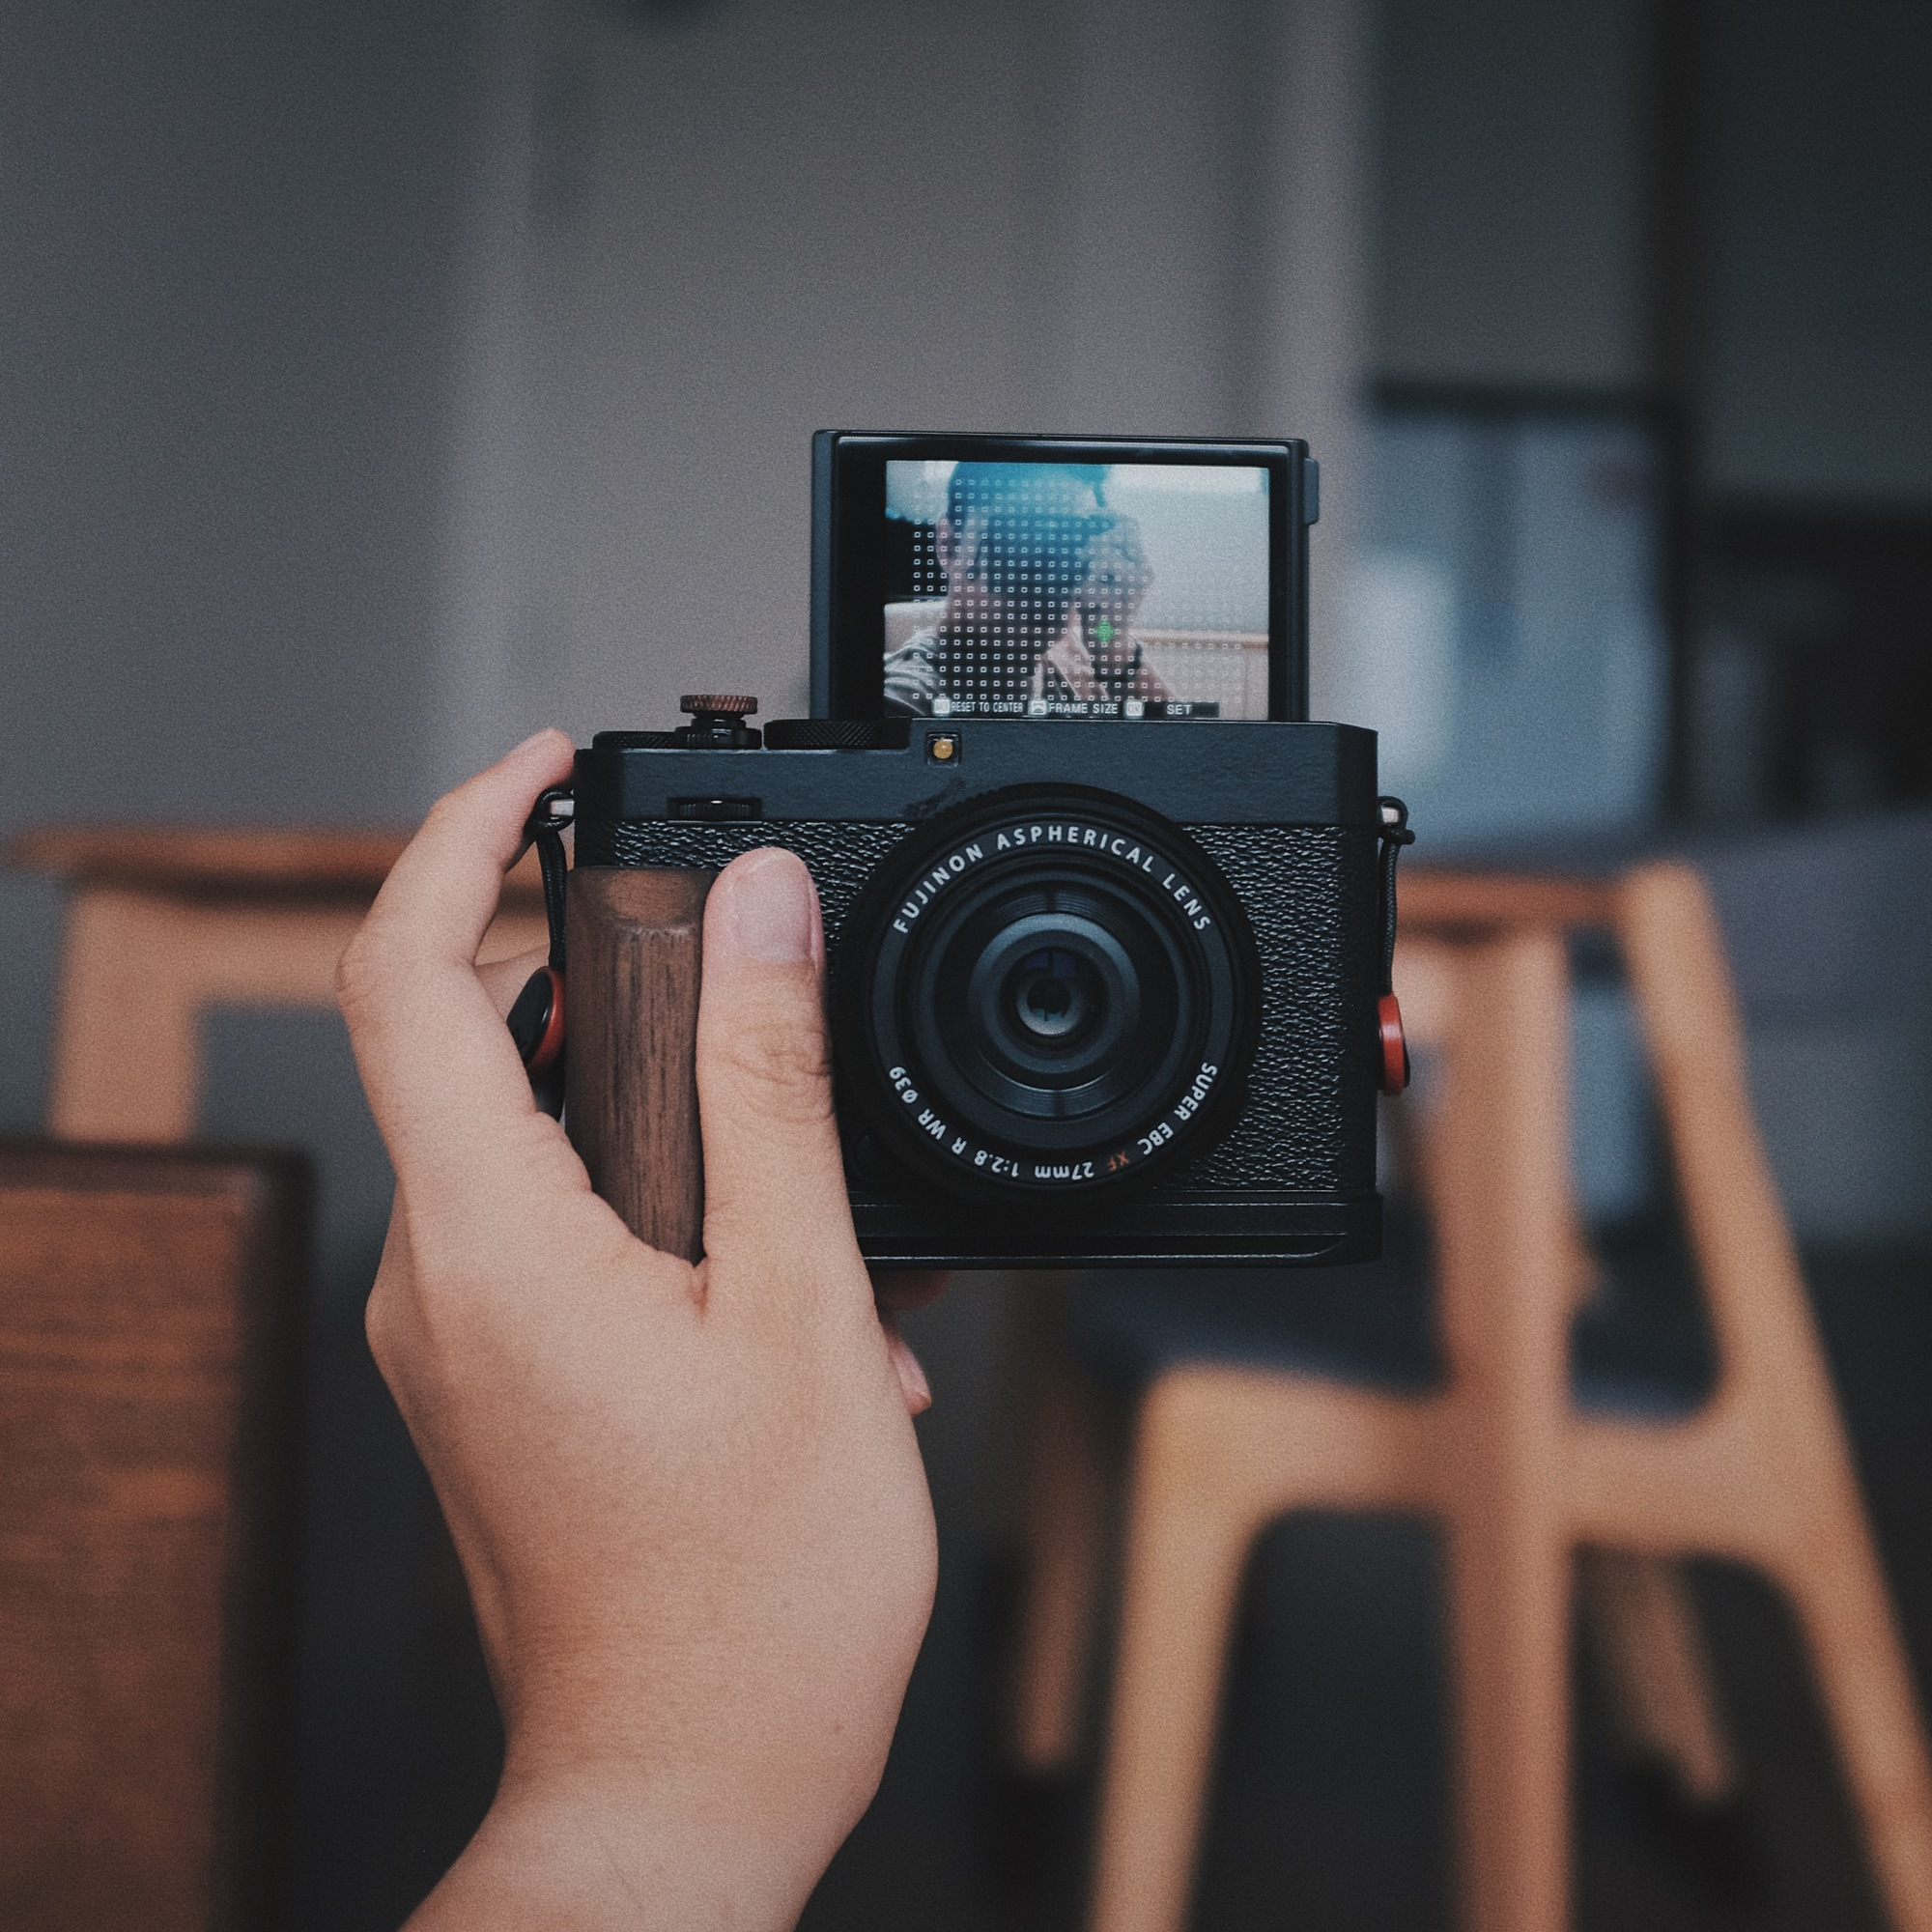
\includegraphics[width=\linewidth]{\envfinaldir/coverpic-prod.jpg}\par
            % \vskip 30pt
            \vfill

            \normalsize\rmfamily\scshape
            \copyright{} The Web Digest Project \hfill\large \envdatestr
        \end{center}
    \end{titlepage}
    % \restoregeometry
}
\newcommand{\simplehref}[1]{%
    \textcolor{blue!80!green}{\href{#1}{#1}}%
}
\renewcommand{\contentsname}{\center\Huge\sffamily\bfseries Contents\par\vskip 20pt}
\newcounter{ipartcounter}
\setcounter{ipartcounter}{0}
\newcommand{\ipart}[1]{
    % \vskip 20pt
    \clearpage
    \stepcounter{ipartcounter}
    \phantomsection
    \addcontentsline{toc}{chapter}{#1}
    % \begin{center}
    %     \Huge
    %     \sffamily\bfseries
    %     #1
    % \end{center}
    % \vskip 20pt plus 7pt
}
\newcounter{ichaptercounter}
\setcounter{ichaptercounter}{0}
\newcommand{\ichapter}[1]{
    % \vskip 20pt
    \clearpage
    \stepcounter{ichaptercounter}
    \phantomsection
    \addcontentsline{toc}{section}{\numberline{\arabic{ichaptercounter}}#1}
    \begin{center}
        \Huge
        \sffamily\bfseries
        #1
    \end{center}
    \vskip 20pt plus 7pt
}
\newcommand{\entrytitlefont}[1]{\subsection*{\raggedright\Large\sffamily\bfseries#1}}
\newcommand{\entryitemGeneric}[2]{
    % argv: title, url
    \parbox{\linewidth}{
        \entrytitlefont{#1}\par\vskip 5pt
        \footnotesize\ttfamily\mdseries
        \simplehref{#2}
    }\vskip 11pt plus 11pt minus 1pt
}
\newcommand{\entryitemGithub}[3]{
    % argv: title, url, desc
    \parbox{\linewidth}{
        \entrytitlefont{#1}\par\vskip 5pt
        \footnotesize\ttfamily\mdseries
        \simplehref{#2}\par\vskip 5pt
        \small\rmfamily\mdseries#3
    }\vskip 11pt plus 11pt minus 1pt
}
\newcommand{\entryitemAp}[3]{
    % argv: title, url, desc
    \parbox{\linewidth}{
        \entrytitlefont{#1}\par\vskip 5pt
        \footnotesize\ttfamily\mdseries
        \simplehref{#2}\par\vskip 5pt
        \small\rmfamily\mdseries#3
    }\vskip 11pt plus 11pt minus 1pt
}
\newcommand{\entryitemHackernews}[3]{
    % argv: title, hnurl, rawurl
    % \parbox{\linewidth}{
    %     \entrytitlefont{#1}\par\vskip 5pt
    %     \footnotesize\ttfamily\mdseries
    %     \simplehref{#3}\par
    %     \textcolor{black!50}{\href{#2}{#2}}
    % }\vskip 11pt plus 11pt minus 1pt
    \begin{minipage}{\linewidth}
            \entrytitlefont{#1}\par\vskip 5pt
            \footnotesize\ttfamily\mdseries
            \simplehref{#3}\par
            \textcolor{black!50}{\href{#2}{#2}}
    \end{minipage}\par\vskip 11pt plus 11pt minus 1pt
}







\begin{document}

\makeheader

\tableofcontents\clearpage




\ipart{Developers}
\ichapter{Hacker News}
\entryitemTwoLinks{Surveillance data challenges what we thought we knew about location tracking}{https://news.ycombinator.com/item?id=45584498}{https://www.lighthousereports.com/investigation/surveillance-secrets/}

\entryitemTwoLinks{Half of America's Voting Machines Are Now Owned by a MAGA Oligarch}{https://news.ycombinator.com/item?id=45584295}{https://dissentinbloom.substack.com/p/half-of-americas-voting-machines}

\entryitemTwoLinks{America Is Sliding Toward Illiteracy}{https://news.ycombinator.com/item?id=45583730}{https://www.theatlantic.com/ideas/archive/2025/10/education-decline-low-expectations/684526/}

\entryitemTwoLinks{What Americans die from vs. what the news reports on}{https://news.ycombinator.com/item?id=45583336}{https://ourworldindata.org/does-the-news-reflect-what-we-die-from}

\entryitemTwoLinks{Beliefs that are true for regular software but false when applied to AI}{https://news.ycombinator.com/item?id=45583180}{https://boydkane.com/essays/boss}

\entryitemTwoLinks{How bad can a \$2.97 ADC be?}{https://news.ycombinator.com/item?id=45582462}{https://excamera.substack.com/p/how-bad-can-a-297-adc-be}

\entryitemTwoLinks{How AI hears accents: An audible visualization of accent clusters}{https://news.ycombinator.com/item?id=45581735}{https://accent-explorer.boldvoice.com/}

\entryitemTwoLinks{GPT-5o-mini hallucinates medical residency applicant grades}{https://news.ycombinator.com/item?id=45581029}{https://www.thalamusgme.com/blogs/cortex-core-clerkship-grades-and-transcript-normalization}

\entryitemTwoLinks{Astronomers 'image' a mysterious dark object in the distant Universe}{https://news.ycombinator.com/item?id=45580699}{https://www.mpg.de/25518363/1007-asph-astronomers-image-a-mysterious-dark-object-in-the-distant-universe-155031-x}

\entryitemTwoLinks{Wireshark 4.6.0 Supports macOS Pktap Metadata (PID, Process Name, etc.)}{https://news.ycombinator.com/item?id=45580315}{https://nuxx.net/blog/2025/10/14/wireshark-4-6-0-supports-macos-pktap-metadata-pid-process-name-etc/}

\entryitemTwoLinks{Let's Not Encrypt (2019)}{https://news.ycombinator.com/item?id=45579968}{https://michael.orlitzky.com/articles/lets\_not\_encrypt.xhtml}

\entryitemTwoLinks{CRISPR-like tools that finally can edit mitochondria DNA}{https://news.ycombinator.com/item?id=45579708}{https://www.nature.com/articles/d41586-025-03307-x}

\entryitemTwoLinks{Pyrefly: Python type checker and language server in Rust}{https://news.ycombinator.com/item?id=45579275}{https://pyrefly.org/?featured\_on=talkpython}

\entryitemTwoLinks{Zoo of array languages}{https://news.ycombinator.com/item?id=45578540}{https://ktye.github.io/}

\entryitemTwoLinks{ADS-B Exposed}{https://news.ycombinator.com/item?id=45578383}{https://adsb.exposed/}

\entryitemTwoLinks{KDE celebrates the 29th birthday and kicks off the yearly fundraiser}{https://news.ycombinator.com/item?id=45578117}{https://kde.org/fundraisers/yearend2025/}

\entryitemTwoLinks{Why the push for Agentic when models can barely follow a simple instruction?}{https://news.ycombinator.com/item?id=45577080}{https://forum.cursor.com/t/why-the-push-for-agentic-when-models-can-barely-follow-a-single-simple-instruction/137154}

\entryitemTwoLinks{Why study programming languages (2022)}{https://news.ycombinator.com/item?id=45576623}{https://people.csail.mit.edu/rachit/post/why-study-programming-languages/}

\entryitemTwoLinks{Copy-and-Patch: A Copy-and-Patch Tutorial}{https://news.ycombinator.com/item?id=45576502}{https://transactional.blog/copy-and-patch/tutorial}

\entryitemTwoLinks{New York Times, AP, Newsmax and others say they won't sign new Pentagon rules}{https://news.ycombinator.com/item?id=45575755}{https://apnews.com/article/pentagon-press-access-defense-department-rules-95878bce05096912887701eaa6d019c6}\ichapter{Phoronix}
\entryitemGeneric{\hskip 0pt{}FSF Announces The LibrePhone Project}{https://www.phoronix.com/news/FSF-LibrePhone-Project}

\entryitemGeneric{\hskip 0pt{}Path Cleared For Nix Package Manager On Fedora With /nix Approved}{https://www.phoronix.com/news/Fedora-Nix-Dir-Approved}

\entryitemGeneric{\hskip 0pt{}Intel Announces "Crescent Island" Inference-Optimized Xe3P Graphics Card With 160GB vRAM}{https://www.phoronix.com/review/intel-crescent-island}

\entryitemGeneric{\hskip 0pt{}Intel Begins Xe Kernel Graphics Driver Enablement For Xe3P With Nova Lake}{https://www.phoronix.com/news/Intel-Xe-3P-NVL-Linux-Start}

\entryitemGeneric{\hskip 0pt{}Yet Another Longtime Linux Driver Maintainer At Intel Has Left}{https://www.phoronix.com/news/Jarkko-Leaving-Intel-Linux}

\entryitemGeneric{\hskip 0pt{}Firefox 145 Beta Released With 32-bit Linux Support Dropped}{https://www.phoronix.com/news/Firefox-145-Beta}

\entryitemGeneric{\hskip 0pt{}Amazon AWS Working On Linux "PCSC" To Help With Dense SR-IOV Deployments}{https://www.phoronix.com/news/AWS-Linux-PCSC-SR-IOV}

\entryitemGeneric{\hskip 0pt{}Linux Mint LMDE 7 Officially Released - Based On Debian 13}{https://www.phoronix.com/news/Linux-Mint-LMDE-7}

\entryitemGeneric{\hskip 0pt{}Linux 6.19 Will Continue With More Rust Graphics Driver Preparations}{https://www.phoronix.com/news/First-DRM-Misc-Next-Linux-6.19}


\ipart{Developers~~~~(zh-Hans)}
\ichapter{Solidot}
\entryitemGeneric{\hskip 0pt{}x86 生态系统顾问团队过去一年的成果}{https://www.solidot.org/story?sid=82544}

\entryitemGeneric{\hskip 0pt{}美国 AI 淘金热下制造业疲软}{https://www.solidot.org/story?sid=82543}

\entryitemGeneric{\hskip 0pt{}日本夏季过去 42 年增加了 3 周}{https://www.solidot.org/story?sid=82542}

\entryitemGeneric{\hskip 0pt{}教宗督促警惕控制算法的人}{https://www.solidot.org/story?sid=82541}

\entryitemGeneric{\hskip 0pt{}大部分开放权重模型都来自中国}{https://www.solidot.org/story?sid=82540}

\entryitemGeneric{\hskip 0pt{}微软终止对 windows 10 的支持}{https://www.solidot.org/story?sid=82539}

\entryitemGeneric{\hskip 0pt{}诺贝尔经济学奖授予了研究创新对经济影响的三名经济学家}{https://www.solidot.org/story?sid=82538}

\entryitemGeneric{\hskip 0pt{}SmartNav 将城市 GPS 精度提升到 10 厘米}{https://www.solidot.org/story?sid=82537}

\entryitemGeneric{\hskip 0pt{}高龄父亲会将更多致病突变遗传给后代}{https://www.solidot.org/story?sid=82536}

\entryitemGeneric{\hskip 0pt{}法拉利宣布首款电动跑车}{https://www.solidot.org/story?sid=82535}

\entryitemGeneric{\hskip 0pt{}Firefox 改进配置文件管理 }{https://www.solidot.org/story?sid=82534}

\entryitemGeneric{\hskip 0pt{}新生儿血液中的超级细菌十分普遍}{https://www.solidot.org/story?sid=82533}

\entryitemGeneric{\hskip 0pt{}流浪天体被发现可能是一颗反复爆发的亚恒星}{https://www.solidot.org/story?sid=82532}

\entryitemGeneric{\hskip 0pt{}金星大气层含水量超预期}{https://www.solidot.org/story?sid=82531}

\entryitemGeneric{\hskip 0pt{}2024 年 3\% 的日本新生儿是外国人}{https://www.solidot.org/story?sid=82530}

\entryitemGeneric{\hskip 0pt{}调查显示美国八成员工抱怨工作损害心理健康}{https://www.solidot.org/story?sid=82529}

\entryitemGeneric{\hskip 0pt{}Linux 6.18-rc1 释出}{https://www.solidot.org/story?sid=82528}

\entryitemGeneric{\hskip 0pt{}LineageOS 23 释出}{https://www.solidot.org/story?sid=82527}

\entryitemGeneric{\hskip 0pt{}同卵双胞胎的 IQ 差异与学校教育相关}{https://www.solidot.org/story?sid=82526}

\entryitemGeneric{\hskip 0pt{}在特朗普宣布加征 100\% 关税前 30 分钟有人对比特币进行巨额做空}{https://www.solidot.org/story?sid=82525}\ichapter{V2EX}
\entryitemGeneric{\hskip 0pt{}[宽带症候群] 还有人用广州电信游戏宽带吗?}{https://www.v2ex.com/t/1165259}

\entryitemGeneric{\hskip 0pt{}[程序员] 有大佬用过 browser use 吗?效果怎么样?}{https://www.v2ex.com/t/1165258}

\entryitemGeneric{\hskip 0pt{}[程序员] 你们撸代码还在 debug 调试吗?}{https://www.v2ex.com/t/1165257}

\entryitemGeneric{\hskip 0pt{}[汽车] 跑高速进服务区要先上厕所,再说其他的……}{https://www.v2ex.com/t/1165256}

\entryitemGeneric{\hskip 0pt{}[问与答] 联想 thinkbook win11 吐个槽}{https://www.v2ex.com/t/1165255}

\entryitemGeneric{\hskip 0pt{}[酷工作] HSBC 校招开始啦}{https://www.v2ex.com/t/1165254}

\entryitemGeneric{\hskip 0pt{}[Stable Diffusion] [求解答] 学习 sd 等精确绘图是否已经过时?}{https://www.v2ex.com/t/1165253}

\entryitemGeneric{\hskip 0pt{}[美国] 最近有从美国回上海的朋友吗?想看看能不能帮忙带点东西}{https://www.v2ex.com/t/1165252}

\entryitemGeneric{\hskip 0pt{}[问与答] 微信输入法越更新越垃圾!模糊音没了,跨设备剪切板也失灵了}{https://www.v2ex.com/t/1165249}

\entryitemGeneric{\hskip 0pt{}[iPhone] Apple 的家庭成员只能是同一个区吗}{https://www.v2ex.com/t/1165248}

\entryitemGeneric{\hskip 0pt{}[问与答] 蓝牙报警(定位)器求推荐}{https://www.v2ex.com/t/1165247}

\entryitemGeneric{\hskip 0pt{}[酷工作] 招兼职求建议}{https://www.v2ex.com/t/1165246}

\entryitemGeneric{\hskip 0pt{}[程序员] 用 Selenium 自动发布今日头条文章失败,有人遇到过类似问题吗?}{https://www.v2ex.com/t/1165245}

\entryitemGeneric{\hskip 0pt{}[Linux] 突发奇想, Linux 软件生态问题}{https://www.v2ex.com/t/1165244}

\entryitemGeneric{\hskip 0pt{}[宽带症候群] TK 域名上传流量异常}{https://www.v2ex.com/t/1165243}

\entryitemGeneric{\hskip 0pt{}[生活] 外地人在大城市长久发展的理由}{https://www.v2ex.com/t/1165242}

\entryitemGeneric{\hskip 0pt{}[分享创造] 快点开源软件趋势}{https://www.v2ex.com/t/1165240}

\entryitemGeneric{\hskip 0pt{}[问与答] lark 邮箱会不会漏收邮件?}{https://www.v2ex.com/t/1165239}

\entryitemGeneric{\hskip 0pt{}[Windows] 今天是 Win10 的圆寂日,以后再也不用升级了。}{https://www.v2ex.com/t/1165238}

\entryitemGeneric{\hskip 0pt{}[问与答] win11 开始菜单 设置 状态栏打不开?但是任务栏应用都可以打开,不想重装系统还有什么办法解决吗}{https://www.v2ex.com/t/1165237}

\entryitemGeneric{\hskip 0pt{}[Apple] 健康 App 导出的 xml 如何转换为 fit 或者 tcx 格式?}{https://www.v2ex.com/t/1165236}

\entryitemGeneric{\hskip 0pt{}[酷工作] [招聘] 我在部门大量 HC,靠谱内推,北京杭州都可以}{https://www.v2ex.com/t/1165234}

\entryitemGeneric{\hskip 0pt{}[分享创造] 做了一个视频翻译工具, 各位有兴趣可以测试下}{https://www.v2ex.com/t/1165233}

\entryitemGeneric{\hskip 0pt{}[Reddit] 😌在 reddit 注册的新账号已发帖就被 shadowbanned 了,吓的我现在注册了新账号也不敢发帖了!}{https://www.v2ex.com/t/1165231}

\entryitemGeneric{\hskip 0pt{}[杭州] 有无保险可以支持门诊的?}{https://www.v2ex.com/t/1165229}

\entryitemGeneric{\hskip 0pt{}[问与答] 用苹果后再也没刷过机,请问下 ios26 能回退吗?}{https://www.v2ex.com/t/1165228}

\entryitemGeneric{\hskip 0pt{}[分享创造] 极简分布式开源 AI 网关 - LLM Gateway 测试版}{https://www.v2ex.com/t/1165227}

\entryitemGeneric{\hskip 0pt{}[生活] 和 v2 老哥们对一对消费情况,对自己的恋爱开销有点疑惑。}{https://www.v2ex.com/t/1165226}

\entryitemGeneric{\hskip 0pt{}[Java] 推广一下自己刚撸的 IDEA 插件—Bean Copy 助手}{https://www.v2ex.com/t/1165225}

\entryitemGeneric{\hskip 0pt{}[问与答] 让 AI 帮我配一台 1 .2w 左右的主机,来了个华硕全家桶, 有什么建议吗?}{https://www.v2ex.com/t/1165223}

\entryitemGeneric{\hskip 0pt{}[酷工作] [长沙-外企] 招聘 Java /QA/Frontend Engineer}{https://www.v2ex.com/t/1165222}

\entryitemGeneric{\hskip 0pt{}[问与答] 2 部手机哪个方案好?}{https://www.v2ex.com/t/1165221}

\entryitemGeneric{\hskip 0pt{}[职场话题] 想请教一下从事 PLC 相关的大哥}{https://www.v2ex.com/t/1165220}

\entryitemGeneric{\hskip 0pt{}[问与答] 基于什么理由 termius 窗口每次关闭打开都要放大一点?}{https://www.v2ex.com/t/1165219}

\entryitemGeneric{\hskip 0pt{}[问与答] 有没有 外语视频 添加 中文配音 的软件?}{https://www.v2ex.com/t/1165218}

\entryitemGeneric{\hskip 0pt{}[Python] 迭代器的实际应用场景是什么?}{https://www.v2ex.com/t/1165216}

\entryitemGeneric{\hskip 0pt{}[Local LLM] [个人项目分享] 写了三篇关于 AI 前沿架构的文章,结合了一些与 AI 对话的独特体验}{https://www.v2ex.com/t/1165215}

\entryitemGeneric{\hskip 0pt{}[推广] 微信返利机器人用哪个}{https://www.v2ex.com/t/1165213}

\entryitemGeneric{\hskip 0pt{}[加密货币] 今天这一波暴跌又是啥情况?}{https://www.v2ex.com/t/1165212}

\entryitemGeneric{\hskip 0pt{}[英雄联盟] theshy}{https://www.v2ex.com/t/1165211}

\entryitemGeneric{\hskip 0pt{}[推广] Poixe AI 流量主计划,将您的影响力转化为收入}{https://www.v2ex.com/t/1165210}

\entryitemGeneric{\hskip 0pt{}[酷工作] 阿里国际急招, Java 开发,缺人,速来。}{https://www.v2ex.com/t/1165208}

\entryitemGeneric{\hskip 0pt{}[Android] 小米狠狠的羡慕 VIVO 用户了}{https://www.v2ex.com/t/1165207}

\entryitemGeneric{\hskip 0pt{}[投资] 有没有亲历的给说说, ibkr 买港股到底会不会被 crs?}{https://www.v2ex.com/t/1165206}

\entryitemGeneric{\hskip 0pt{}[问与答] Mouse Without Borders(无界鼠标) 已经开源了,有人做跨平台 mac/安卓客户端么}{https://www.v2ex.com/t/1165205}

\entryitemGeneric{\hskip 0pt{}[问与答] pixel 手机可以存多少个 esim 号码}{https://www.v2ex.com/t/1165203}

\entryitemGeneric{\hskip 0pt{}[Linux] 使用 qemu-img 创建 raw 格式的磁盘文件,为什么前 4KB 要用 0 填充?}{https://www.v2ex.com/t/1165202}

\entryitemGeneric{\hskip 0pt{}[随想] 每个人都有自己的逻辑闭环,失去这点,则无法冷静下来}{https://www.v2ex.com/t/1165200}

\entryitemGeneric{\hskip 0pt{}[分享创造] 做了个垃圾 ``卖价值'',然后有了第一个客户,激动!}{https://www.v2ex.com/t/1165199}

\entryitemGeneric{\hskip 0pt{}[求职] 深圳 4 年 golang 服务端开发求职🙏}{https://www.v2ex.com/t/1165198}


\ipart{Generic News}







\clearpage
\leavevmode\vfill
\footnotesize

Copyright \copyright{} 2023-2025 Neruthes and other contributors.

This document is published with CC BY-NC-ND 4.0 license.

The entries listed in this newsletter may be copyrighted by their respective creators.

This newsletter is generated by the Web Digest project.

The newsletters are also delivered via Telegram channel \CJKunderline{\href{https://t.me/webdigestchannel}{https://t.me/webdigestchannel}}.\\
RSS feed is available at \CJKunderline{\href{https://webdigest.pages.dev/rss.xml}{https://webdigest.pages.dev/rss.xml}}.

This newsletter is available in PDF at
\CJKunderline{\href{https://webdigest.pages.dev/}{https://webdigest.pages.dev/}}.

The source code being used to generate this newsletter is available at\\
\CJKunderline{\href{https://github.com/neruthes/webdigest}{https://github.com/neruthes/webdigest}}.

This newsletter is also available in
\CJKunderline{\href{http://webdigest.pages.dev/readhtml/\envyear/WebDigest-20251015.html}{HTML}} and
\CJKunderline{\href{https://github.com/neruthes/webdigest/blob/master/markdown/\envyear/WebDigest-20251015.md}{Markdown}}.


\coverpic{https://unsplash.com/photos/woman-with-glasses-in-front-of-chalkboard-QafdD54AgCo}{Vitaly Gariev}


\end{document}
